\documentclass[draftclsnofoot, onecolumn, compsoc, 10pt]{IEEEtran}

\title{\huge Software Requirements Specifications}
\author{Oregon State University\\CS 461\\2017-2018\\\\Prepared By:\\ Kyle Prouty\\Hayden Anderson\\Lucien Tamno}

\usepackage{titling}
\usepackage[margin=0.75in]{geometry}
\usepackage{graphicx}
\graphicspath{ {images/} }
\linespread{1.0}
\parindent=0.0in
\parskip=0.2in

\begin{document}
\begin{titlingpage}
    \maketitle 
\end{titlingpage}

\tableofcontents
\pagebreak

\section{Introduction}
\subsection{Purpose}
The purpose of this document is to layout and define the objective and details of the framework. This document will specify an overall description, specific requirements, and software system attributes of the framework. The intended audience for this document includes any relevant stakeholders. 

\subsection{Scope} % HAYDEN here
The main goal of this framework will be to allow a user to input an objective into a collection of nodes. These nodes will then carryout the objective based on the services required. The services needed to finish the job will propagate through the system to find the nodes that can carryout each service. Once each service in an objective has a node that can carry them out. The node that received the user input will output where the piece(s) of the objective are being completed. The framework will be able to (re)direct services and jobs away from established security threatened nodes.  
% \centering{
% 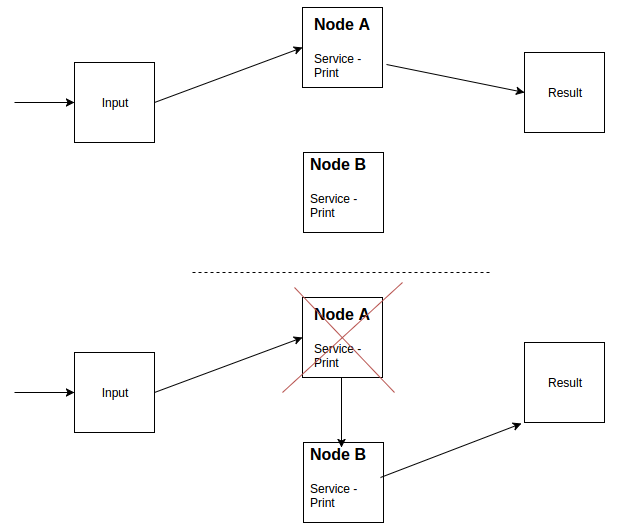
\includegraphics[scale=0.4]{img_1}
% }

\subsection{Definitions, Acronyms, Abbreviations}
\bgroup
\def\arraystretch{1.5}
\resizebox{\textwidth}{!}{
\begin{tabular}{| p{10.0cm} | p{10.0cm} |}
\hline
\bf{Term} & \bf{Definition}\\ 
\hline
Stake Holder  & User of the framework \\
\hline
GUI  & Graphical User Interface  \\ 
\hline
User  & The person who would use this at its completion that doesn’t know how it works   \\
\hline
IoT  & Internet of Things  \\ 
\hline
Node  & Our built device that acts as a layer between IoT enabled machines and other nodes \\ 
\hline
Social Device  & An IoT enabled device that can connect and (talk) with other IoT devices.  \\ 
\hline
MVC  & Model View Controller; A software architecture for implementing an interface for the user  \\ 
\hline
Docker &  A container of isolated code \\
\hline
Linux & An open-source operating system \\
\hline
WLAN & Wireless local area network \\
\hline
MQTT & Message Queue Telemetry Transport \\
\hline
\end{tabular}
}
\egroup

\subsection{References}
IEEE. IEEE Std 830-1998 IEEE Recommended Practice for Software Requirements Specifications. IEEE Computer Society,1998.

\subsection{Overview}
In the next section of this document, Overall Description, will give an overview of software dependencies, the intended function, characteristics, constraints, and assumptions of the framework. This section is geared more towards giving a more high level examination of the framework. The third section, Specific Requirements, is intended for more of a technical audience who would be familiar with the technical aspects and relevant terminology of this framework. 

\section{Overall Description}
\subsection{Product Perspective}
{\centering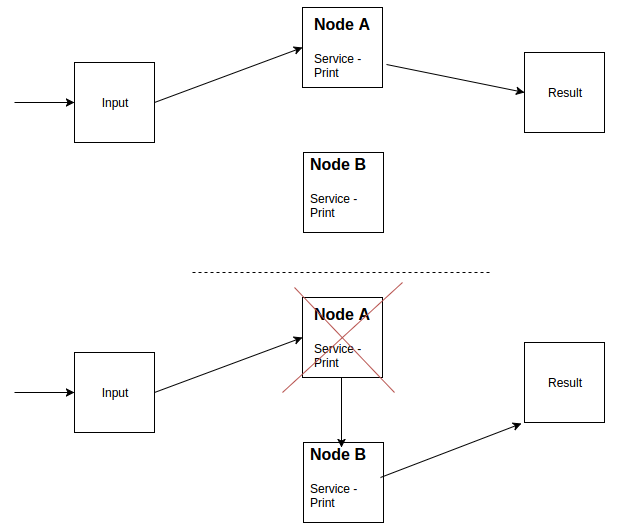
\includegraphics[scale=0.4]{img_1}}

\subsubsection{System Interfaces}
The primary system interface will be the Linux operating system. This framework will interact with the Linux operating system in order to utilize its services.

\subsubsection{User Interfaces}
\begin{itemize}
\item A command line based interface used to connect to a specific node to change configuration setting. \\ 
\item A web based gui that will interface between an administrator and the nodes. This graphical interface is used to show the nodes in the framework, the services each node offers, and the nodes connections with each other.\\ 
\item A web based gui that will interface between a user and the nodes. This graphical interface is used to let a user upload a file into the collection of nodes and view the status of the result.
\end{itemize}

\subsubsection{Hardware Interfaces}
This framework will use a combination of various micro-controllers. These micro-controllers must have the functionality to communicate with WLAN communication protocols.

\subsubsection{Software Interfaces}
Nodes will only interact with the Linux operating system. Users will interact with a web based browser.

\subsubsection{Communications Interfaces}
The Network Protocol that is required by this framework is Ethernet with the communication protocols, TCP/IP and WLAN.

\subsubsection{Memory constraints}
The framework is only constrained to what the hardware that is used will allow.
 
\subsubsection{Operations}
There will be three modes of operation within the user organization. The main mode of operation is the device mode. This mode will operate exclusively in the background. Next is the user mode which will be input and output operations. Third there will be an administer mode which will allow the sending of commands and the viewing of state and status.

\subsubsection{Site Adaptation Requirements}
No site adaptations required.


\subsection{Product Functions}


\subsection{User Characteristics} 
The users of this framework will be our relevant stakeholders. These users will have had some level of formal technical education.

\subsection{Constraints}
This framework must not have a singular node that is always the leader. Each individual node must be able to lead the framework on decisions required. Nodes cannot utilize an external database for its inner information structure. Nodes cannot exchange information by using an external database.

\subsection{Assumptions and Dependencies}
This document and current requirements assume that each hardware device we use can handle concurrency and has wifi capabilities. Each device has the memory and storage large enough to fit our docker image and run. Each physical device is able to handle a small simple gui.

\subsection{Apportioning of Requirements}
Refer to Gantt chart for this information.\\\\ 
{\centering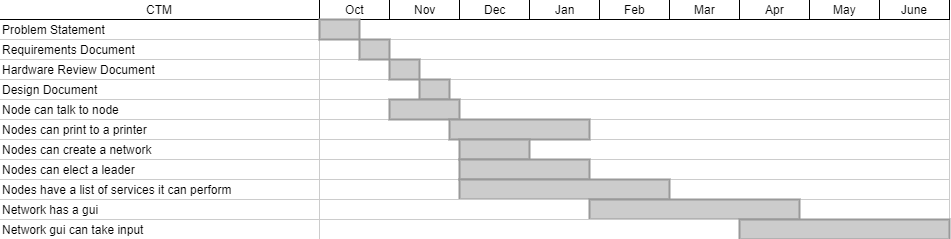
\includegraphics[scale=0.4]{chart}}


\section{Specific Requirements}
\subsection{External Interfaces}
All interfaces will be external.

\subsection{Functions}
The system shall...

\subsection{Performance Requirements}
There are to be up to 5 nodes supported in a network. Each objective received by the network from the user are to be able to start 90 of the services required by the objective given. Only one user will be able to use the gui or terminal at a time (more for a stretch goal?). Only one objective can be handled by the network at a time (more for a stretch goal?). No objectives can be stacked onto existing objectives to be performed consecutively (remove for stretch goal?). Each node will be able to support up to 10 services (make unlimited and/or match to it’s connected IoT device for a stretch goal).

\subsection{Logical Database Requirements}
There are no database requirements. 

\subsection{Design Constraints}
There is not an external database to which the nodes should be writing to or retrieving from to be able to be a part of the nodal network or carry out objectives.

\subsection{Standards Compliance}
This framework will need to stay compliant with IEEE WLAN and MQTT standards.

\section{Software System Attributes}
\subsection{Reliability}
The reliability of this framework will be measured by the ability to connect and send commands to it. 

\subsection{Security}
Nodes on this network will be password protected and only accept authorized users.

\subsection{Maintainability}
Code will be well commented and readable to another software developer. A MVC design scheme will be implemented. File structure will be well organized and self explanatory to navigate.


\subsection{Portability}
This framework will be fully portable to any system that can run a Docker container. 

\subsection{Specific Requirements}
\subsubsection{User Interfaces}
\subsubsection{Hardware Interfaces}
\subsubsection{Software Interfaces}
\subsubsection{Communication Interfaces}
\subsubsection{Other Requirements} 

\end{document}